%!TEX root = <main.tex>
\section{Preliminaries and Overview}\label{sec:preliminaries}
In this section, we first formally state the problem and explain our assumptions.
Then we formalize the internals of critical layers in a Deep CNN for the purpose of proposing our \textit{incremental inference} approach in Section 4.
\eat{
Finally we briefly explain the Structural Similarity Index (SSIM) which is used to quantify the quality of the generated sensitivity heat maps.
}

\subsection{Problem Statement and Assumptions}

\begin{table}[t]
  \centering
  \caption{Symbols used in the Preliminaries Section}
  \scalebox{0.8}{\begin{tabular}{p{2cm}p{7.5cm}}
    \toprule
    \textbf{Symbol} & \textbf{Meaning}\\
    \midrule \midrule
    $^l\mathcal{I} (^{img}\mathcal{I})$ & Input activation volume of the $l^{th}$ layer (Input Image)\\
    \midrule
    $^l\mathcal{O}$ & Output activation volume of the $l^{th}$ layer\\
    \midrule
    $^lC_{\mathcal{I}},{}^lH_{\mathcal{I}},{}^lW_{\mathcal{I}}$ & Depth, height, and width of $l^th$ layer Input\\
    \midrule
    $^lC_{\mathcal{O}},{}^lH_{\mathcal{O}},{}^lW_{\mathcal{O}}$ & Depth, height, and width of $l^{th}$ layer Output\\
    \midrule
    $^l\mathcal{K}_{conv}$ & Convolution filter kernels for the $l^{th}$ layer\\
    \midrule
    $^l\mathcal{B}_{conv}$ & Convolution bias value vector for the $l^{th}$ layer\\
    \midrule
    $^l\mathcal{K}_{pool}$ & Pooling filter kernel for the $l^th$ layer\\
    \midrule
    $^lH_{\mathcal{K}},{}^lW_{\mathcal{K}}$ & Height and width of the filter kernel for the $l^{th}$ layer\\
    \midrule
    $^lS$$\equiv$$(^lS_x,{}^lS_y)$ & Filter kernel patch striding amount for the $l^{th}$ layer ($^lS_x$ and $^lS_y$ corresponds to width and height dimensions)\\
    \midrule
    $^lP$$\equiv$$(^lP_x,{}^lP_y)$ & Padding amount for the $l^{th}$ layer ($^lP_x$ and $^lP_y$ corresponds to padding along width and height dimensions)\\
    \midrule
    % $Q (Q_{inc})$ & Total FLOPS count with full (incremental) inference\\
    % \midrule
    % $L$ & Set of convolution layers in a CNN\\
    % \midrule
    $\mathcal{P}$ & Occluding patch in RGB format\\
    \midrule
    $^\mathcal{P}S$ & Occluding patch striding amount\\
    \midrule
    % $^{img}\mathcal{I}_{x,y}$ & Modified image by superimposing $\mathcal{P}$ on top of $^{img}\mathcal{I}$ such that the top left corner of $\mathcal{P}$ is positioned at $x,y$ location of $^{img}\mathcal{I}$\\
    % \midrule
    $M$ & Heat map produced by the occlusion experiment\\
    \midrule
    $H_M,W_M$ & Height and width of $M$\\
    \midrule
    $f$ & Fine-tuned CNN which takes in an input image and outputs a probability distribution over the class labels\\
    \midrule
    $L$ & Class label predicted by $f$ for the original image $^{img}\mathcal{I}$\\
    \midrule
    $G$ & Set of occluding patch superimposition positions on $^{img}\mathcal{I}$ in (x,y) format\\
    \midrule
    $\bm\circ_{x,y}$ & Superimposition operator. $A~\circ_{x,y}~B$, superimposes $B$ on top of $A$ starting off at $(x,y)$ position\\
    \bottomrule
  \end{tabular}}
\label{table:preliminaries_symbols}
\end{table}


We are given a CNN $f$, an image $^{img}\mathcal{I}$ on which the occlusion experiment needs to be run, the predicted class label $L$ for $^{img}\mathcal{I}$, an occluding patch $\mathcal{P}$ in RGB format, and occluding patch striding amount $^{\mathcal{P}}S$.
In the interactive case \system~ expects the user to also provide a set of interested occluding patch positions $G$.
In the non-interactive scenario \system~ uses the user provided $^\mathcal{P}S$ value to initialize $G$ to the all possible occluding positions.
The occlusion experiment workload is to generate a 2-D heat map $M$ with values corresponding to the coordinates in $G$ contain the predicted probability for $L$ by $f$ for the occluded image $^{img}\mathcal{I}^{'}_{x,y}$ and zero otherwise.
More precisely, we can state the workload using the following set of logical statements:


\begin{align}
\label{eqn:mheight}
W_M =&~ \lfloor(\texttt{width}(^{img}\mathcal{I}) - \texttt{width}(\mathcal{P}) + 1)/^\mathcal{P}S\rfloor\\
\label{eqn:mwidth}
H_M =&~ \lfloor(\texttt{height}(^{img}\mathcal{I}) - \texttt{height}(\mathcal{P}) + 1)/^\mathcal{P}S\rfloor\\
M \in&~ \mathcal{\rm I\!R}^{H_M \times W_M}\\
\forall~ x,y \in&~ G:\\
\label{eqn:patchimpose}
& ^{img}\mathcal{I}^{'}_{x,y} \leftarrow {}^{img}\mathcal{I} ~ \bm\circ_{x,y} ~ \mathcal{P} \\
\label{eqn:outputval}
& M[x,y] \leftarrow f(^{img}\mathcal{I}^{'}_{x,y})[L]
\end{align}




Step (\ref{eqn:mheight}), and (\ref{eqn:mwidth}) calculates the dimensions of the generated heat map $M$ which is dependent on the dimensions of $^{img}\mathcal{I}$, $\mathcal{P}$, and $^\mathcal{P}S$.
Step (\ref{eqn:patchimpose}) superimposes $\mathcal{P}$ on $^{img}\mathcal{I}$ with its top left corner placed on the (x,y) location of $^{img}\mathcal{I}$.
Step (\ref{eqn:outputval}) calculates the output value at the (x,y) location by performing CNN inference for $^{img}\mathcal{I}^{'}_{x,y}$ using $f$ and taking the predicted probability for the label $L$.
Step \ref{eqn:patchimpose} and \ref{eqn:outputval} are run for all occluding patch position values in $G$.
In the non-interactive case $G$ is initialized to $G = [0, H_M) \times [0, W_M)$.
In the interactive case it is possible that human operator would provide multiple $G$s, one after the other, for which the system has to evaluate iteratively.

We assume that $f$ is a CNN from a roster of well-known CNNs (currently, VGG 16 layer version, ResNet 18 layer version, and Inception version 3).
This is a reasonable start since most recent CNN based image recognition applications use only such well-known CNNs from model zoos \cite{caffemodelzoo, tfmodelzoo}.
Nevertheless, our work is orthogonal to the specifics of a particular architecture and the proposed approaches can be easily extended to any architecture.
We leave support for arbitrary CNNs to future work.

\subsection{Deep CNN Internals}
Input and output of individual layers in a Deep CNN except for Fully-Connected ones are arranged into three-dimensional volumes which have a width, height, and depth.
For example an RGB input image of 224$\times$224 spatial sizes can be considered as an input volume having a width and height of 224 and a depth of 3 (corresponding to 3 color channels).
Every non Fully-Connected layer will take in an input volume and transform it into another volume.
A Fully-Connected layer takes in a vector or flattened activation volume as input and transforms it into another vector.
For our purpose, these transformations can be broadly divided into three categories based on how they operate spatially:

\begin{figure*}[t]
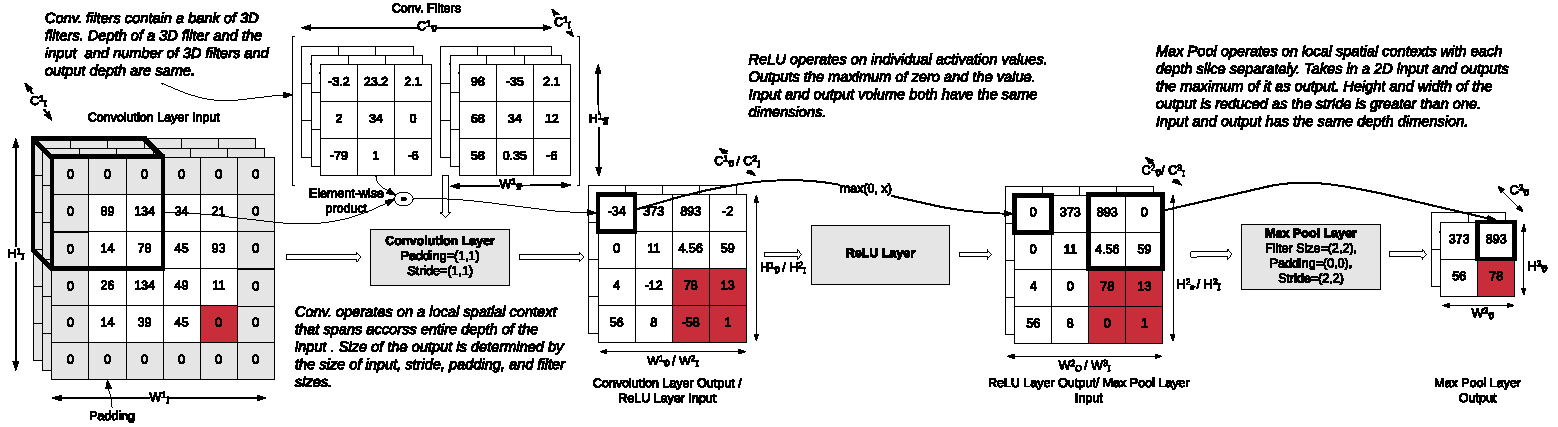
\includegraphics[width=\textwidth]{images/cnn_simplified}
\caption{Simplified representation of selected layers of a Deep CNN. For simplicity addition of bias is not shown in the Convolution transformation. The values marked in red show how a small spatial update in the first input would propagate through subsequent transformation. Notation is explained in Table ~\ref{table:preliminaries_symbols}.}
\label{fig:cnn_simplified}
\end{figure*}

\begin{itemize}
    \item Transformations that operate at the granularity of a global context.
    \begin{itemize}
     \item E.g. Fully-Connected
    \end{itemize}
	\item Transformations that operate at the granularity of individual  spatial locations.
	\begin{itemize}
	 \item E.g. ReLU, Batch Normalization
	\end{itemize}
	\item Transformations that operate at the granularity of a local spatial context.
	\begin{itemize}
	 \item E.g. Convolution, Pooling
	\end{itemize}
\end{itemize}

\vspace{2mm}
\noindent \textbf{Transformations that operate at the granularity of a global context.} These transformations operate on a global context or in other words, does not take into account the spatial information.
Fully-Connected layer, which is the only global context transformation in a CNN, takes in an input vector and performs a vector-matrix multiplication with a weight matrix and produces an output.
As they perform one bulk transformation there is no opportunity for exploiting redundancies.
The computational cost of a Full-Connected transformation is proportional to the product of the size of the input and output vectors.
Fully-Connected layers are used as the last or last few layers in a CNN and only accounts for a small fraction of the total computational cost.

\vspace{2mm}
\noindent \textbf{Transformations that operate at the granularity of individual  spatial locations.} These transformations essentially perform a $map(.)$ function on each individual activation value (see Figure \ref{fig:cnn_simplified} (b)).
Hence the output will have the same dimensions as input.
The computational cost incurred by these transformations is proportional to the volume of the input (or output).
However, with incremental spatially localized updates in the input, such as placing an occlusion patch, only the updated region is needed to be recalculated.
Extending these transformations to become change aware is straightforward.
The computational cost of the change aware incremental transformation is proportional to the volume of the modified region.

\eat{
With incremental spatially localized updates in the input, such as placing an occlusion patch, both types of transformations that operate at the granularity of individual spatial locations and local spatial contexts provide opportunities for exploiting redundancy.
Extending point transformations to become redundancy aware is straightforward. However, with local context transformations, such as Convolution and Pooling, this extension is non-trivial due to the overlapping nature of the spatial contexts. A simplified representation of point transformations and local context transformations is shown in Figure \ref{fig:cnn_simplified}.
It also shows how different types of transformations would propagate a spatially localized change (marked in red) in the input.
We next formally define the transformations of Convolution and Pooling layers and also the relationship between input and output dimensions.
}

\vspace{2mm}
\noindent \textbf{Transformations that operate at the granularity of a local spatial context.}
With incremental spatially localized updates in the input, transformations that operate at the granularity of a local spatial context also provide opportunities for exploiting redundancy and can be made change aware.
However, with local context transformations, such as Convolution and Pooling, this extension is non-trivial due to the overlapping nature of the spatial contexts.
% Convolution layers are the most important type of layer in the CNN architecture which also contributes to most of the computational cost.
Each Convolution layer can have $^lC_{\mathcal{O}}$ 3-D filter kernels organized into a 4-D array $^l\mathcal{K}_{conv}$ with each having a smaller spatial width $^lW_\mathcal{K}$ and height $^lH_\mathcal{K}$ compared to the width $^lW_{\mathcal{I}}$ and height $^lH_{\mathcal{I}}$ of the input volume $^l\mathcal{I}$, but has the same depth $^lC_{\mathcal{I}}$.
During inference, $c^{th}$ filter kernel is strided along the width and height dimensions of the input and a 2-D activation map $^cA=(^ca_{y,x})\in \mathcal{\rm I\!R}^{^lH_{\mathcal{O}} \times~ ^lW_{\mathcal{O}}}$ is produced by taking element\-wise product between the kernel and the input and adding a bias value as per Equation \ref{eqn:elementwise_product}.
The computational cost of each of these individual element-wise product is proportional to the volume of the filter kernel.
Finally, these 2-D activation maps are stacked together along the depth dimension to produce an output volume $^{l}\mathcal{O} \in \mathcal{\rm I\!R}^{^lC_\mathcal{O} \times {}^lH_{\mathcal{O}} \times~ ^lW_{\mathcal{O}}}$ as per Equation \ref{eqn:conv_operator}.
A simplified representation of Convolution transformation is shown in Figure \ref{fig:cnn_simplified} (a).


\begin{align}
\label{eqn:elementwise_product}
\begin{split}
^ca_{y,x} =& \sum_{k=0}^{^lC_\mathcal{I}} \sum_{j=0}^{^lH_\mathcal{K}-1} \sum_{i=0}^{^lW_\mathcal{K}-1} {}^l\mathcal{K}_{conv}[c, k, j, i] \\
& \quad \times {}^l\mathcal{I}[k,y-\floor{\frac{^lH_\mathcal{K}}{2}}+j,x-\floor{\frac{^lW_\mathcal{K}}{2}}+i] \\
& \quad + {}^l\mathcal{B}_{conv}[c]
\end{split}
\end{align}

\begin{align}
\label{eqn:conv_operator}
\begin{split}
^l\mathcal{O} = [^0A, {}^1A, ... , {}^{^lC_\mathcal{O}-1}A]
\end{split}
\end{align}


\eat{
\begin{align}
\begin{split}
\text{Input Volume}:&~ \mathcal{I} \in \mathcal{\rm I\!R}^{C_{\mathcal{I}} \times H_{\mathcal{I}} \times W_{\mathcal{I}}}\\
\text{Convolution Filters}:&~ \mathcal{K}_{conv} \in \mathcal{\rm I\!R}^{C_{\mathcal{O}} \times C_{\mathcal{I}} \times H_{\mathcal{K}} \times W_{\mathcal{K}}}\\
\text{Convolution Bias Vector}:&~ \mathcal{B}_{conv} \in \mathcal{\rm I\!R}^{C_{\mathcal{O}}}\\
\text{Output Volume}:&~ \mathcal{O} \in \mathcal{\rm I\!R}^{C_{\mathcal{O}} \times H_{\mathcal{O}} \times W_{\mathcal{O}}}
\end{split}
\end{align}

\begin{equation}
\label{eqn:conv_operator}
\begin{split}
\mathcal{O}[c,y,x] &= \sum_{k=0}^{C_{\mathcal{I}}} \sum_{j=0}^{H_\mathcal{K}-1} \sum_{i=0}^{W_\mathcal{K}-1} \mathcal{K}_{conv}[c, k, j, i] \\ & \quad \quad \quad \times \mathcal{I}[k,y-\floor{\frac{H_\mathcal{K}}{2}}+j,x-\floor{\frac{W_\mathcal{K}}{2}}+i] + \mathcal{B}[c]
\end{split}
\end{equation}
}

Pooling can also be thought as a Convolution operation with a fixed (i.e. not learned) 2-D filter kernel $^l\mathcal{K}_{pool}$.
But unlike Convolution, Pooling operates independently on each depth slice of the input volume.
% The two main variations of pooling layers are max pooling (takes the maximum value from the local spatial context) and average (takes the average value from the local spatial context) pooling.
A Pooling layer takes a 3-D activation volume $^l\mathcal{O}$ having a depth of $^lC$, width of $^lW_{\mathcal{I}}$, and height of $^lH_{\mathcal{I}}$ as input and produces another 3-D activation volume $^l\mathcal{O}$ which has the same depth of $^lC$, width of $^lW_{\mathcal{O}}$, and height of $^lH_{\mathcal{O}}$ as the output.
Pooling kernel is generally strided with more than one pixel at a time and hence $^lW_{\mathcal{O}}$ and $^lH_{\mathcal{O}}$ are generally smaller than $^lW_{\mathcal{I}}$ and $^lH_{\mathcal{I}}$.
A simplified representation of Pooling transformation is shown in Figure \ref{fig:cnn_simplified} (c).
% Similar to Convolution, Pooling operation can be formally defined as follows:

% \begin{align}
% \text{Pool Filters}:&~ \mathcal{K}_{pool} \in \mathcal{\rm I\!R}^{H_{\mathcal{K}} \times W_{\mathcal{K}}}
% \end{align}

% \begin{equation}
% \label{eqn:pool_operator}
% \begin{split}
% \mathcal{O}[c,y,x] &= \sum_{j=0}^{H_\mathcal{K}-1} \sum_{i=0}^{W_\mathcal{K}-1} \mathcal{K}_{pool}[j, i] \\ & \quad \quad \quad \times \mathcal{I}[c,y-\floor{\frac{H_\mathcal{K}}{2}}+j,x-\floor{\frac{W_\mathcal{K}}{2}}+i]
% \end{split}
% \end{equation}


\vspace{2mm}
\noindent \textbf{Relationship between Input and Output Spatial Sizes.}
The output volume's spatial sizes $^lW_{\mathcal{O}}$ and $^lH_{\mathcal{O}}$ are determined by the spatial sizes of the input volume $^lW_{\mathcal{I}}$ and $^lH_{\mathcal{I}}$, spatial sizes of the filter kernel $^lW_\mathcal{K}$ and $^lH_\mathcal{K}$ and two other parameters: \textbf{stride} $^lS$ and \textbf{padding} $^lP$.
Stride is the amount of pixel values used to slide the filter kernel at a time when producing a 2-D activation map.
It is possible to have two different values with one for the width dimension $^lS_x$ and one for the height dimension $^lS_y$.
Generally $^lS_x \leq {}^lW_\mathcal{K}$ and $^lS_y \leq {}^lH_\mathcal{K}$.
In Figure \ref{fig:cnn_simplified} Convolution transformation uses a stride value of 1 and Pool transformation uses a stride value of 2 for both dimensions.
Sometimes in order to control the spatial size of the output activation map to be same as the input activation map, one needs to pad the input feature map with zeros around the spatial border.
Padding $^lP$ captures the amount of zeros that needs to be added.
Similar to the stride $^lS$, it is possible to have two separate values for padding with one for the width dimension $^lP_x$ and one for the height dimension $^lP_y$.
In Figure \ref{fig:cnn_simplified} Convolution transformation pads the input with one line of zeros from both dimensions.
With these parameters defined, the width (similarly height) of the output activation volume can be defined as follows:

\begin{align}
\begin{split}
^lW_{\mathcal{O}} = (^lW_{\mathcal{I}} - {}^lW_\mathcal{K} + 1 + 2\times {}^lP_x)/^lS_x \\
% ^lH_{\mathcal{O}} = (^lH_{\mathcal{I}} - ^lH_\mathcal{K} + 1 + 2\times ^lP_y)/^lS_y
\end{split}
\end{align}

\vspace{2mm}
\noindent \textbf{Estimating the Computational Cost of Deep CNNs.}
Deep CNNs are highly compute intensive and out of the different types of layers Convolution layers contribute to $90\%$ (or more) of the computation.
Hence we can estimate the computational cost of a Deep CNN by counting the number of fused multiply-add (FMA) floating point operations (FLOPs) required by Convolution layers for a single forward inference.
% and ignore the computational cost of other layers (e.g. Pooling, Fully-Connected).

For example, applying a Convolution filter having the dimensions of ($^lC_\mathcal{I}$, $^lH_{\mathcal{K}}$, $^lW_{\mathcal{K}}$) to a single spatial context will require $^lC_{\mathcal{I}} \times~ ^lH_{\mathcal{K}} \times~ ^lW_{\mathcal{K}}$ many FLOPs, each corresponding to a single element-wise multiplication.
Thus, the total amount of computations $^lQ$ required by that layer in order to produce an output $\mathcal{O}$ having dimensions $^lC_{\mathcal{O}} \times~ ^lH_{\mathcal{O}} \times~ ^lW_{\mathcal{O}}$, and the total amount of computations $Q$ required to process the entire set of convolution layers $L$ in the CNN can be calculated as per Equation \ref{eqn:full_local} and ~\ref{eqn:full_all}.
However, in the case of incremental updates only a smaller spatial patch having a width $^lW_\mathcal{P}$ ($^lW_\mathcal{P}<={}^lW_{\mathcal{O}}$) and height $^lH_\mathcal{P}$ ($^lH_\mathcal{P}<={}^lH_{\mathcal{O}}$) is needed to be recomputed.
The amount of computations required for the incremental computation $^lQ_{inc}$ and total amount of incremental computations $Q_{inc}$ required for the entire set of convolution layers $L$ will be smaller than the above full computation values and can be calculated as per Equation ~\ref{eqn:inc_local} and ~\ref{eqn:inc_all}.
Notice that in both of the above formulations computational cost calculation takes into account the spatial sizes of the output or the output patch.
The output spatial sizes can be determined using the spatial sizes of the input and other parameters as shown in the previous Section.
In Section \ref{sec:optimizer} we show that the spatial sizes of the output patch can also be predetermined using the input patch spatial sizes.

Based on the above quantities we define a new metric named \textit{theoretical speedup} R, which is the ratio between the total full computational cost $Q$ and total incremental computation cost $Q_{inc}$ (see Equation ~\ref{eqn:redundancy_ratio}).
This ratio essentially acts as a surrogate for the theoretical upper-bound for computational and runtime savings that can be achieved by applying incremental computations to deep CNNs.

\begin{align}
\label{eqn:full_local}
^lQ = (^lC_{\mathcal{I}} \times&~ ^lH_{\mathcal{K}} \times{}^lW_{\mathcal{K}}) \times~ (^lC_{\mathcal{O}} \times~ ^lH_{\mathcal{O}} \times{}^lW_{\mathcal{O}})\\
\label{eqn:full_all}
Q =&~ \sum_{l \in L}{}^lQ\\
\label{eqn:inc_local}
^lQ_{inc} = (^lC_{\mathcal{I}} \times&~ ^lH_{\mathcal{K}} \times~ ^lW_{\mathcal{K}}) \times~ (^lC_{\mathcal{O}} \times~ ^lH_{\mathcal{P}} \times~ ^lW_{\mathcal{P}})\\
\label{eqn:inc_all}
Q_{inc} =&~ \sum_{l \in L} ^lQ_{inc}\\
\label{eqn:redundancy_ratio}
R =&~ \frac{Q}{Q_{inc}}
\end{align}


\eat{
\subsection{Estimating the Quality of Generated Approximate Heat Maps}

When applying approximate inference optimizations \system~ sacrifices the the accuracy/quality of the generated heat map in favor of faster execution.
To measure this drop of accuracy we use Structural Similarity (SSIM) Index~\cite{wang2004image} which is one of the widely used approaches to measure the \textit{human perceived difference} between two similar images.
When applying SSIM index we treat the original heat map as the reference image with no distortions and the perceived image similarity of the \system~generated heat map is calculated with reference to it.
The generated SSIM index is a value between $-1$ and $1$, where $1$ corresponds to perfect similarity.
% It is important to note that, even though SSIM index value of 1 corresponds to perfect similarity, other values doesn't necessarily imply same level of perceived quality across different image pairs.
% However, if the original images are closely similar, such as in chest X-ray images, it can be assumed that this condition will hold.
Typically SSIM index values in the range of $0.90-0.95$ are used in practical applications such as image compression and video encoding as at the human perception level they produce indistinguishable distortions.
For more details on SSIM Index method, we refer the reader to the original SSIM Index paper~\cite{wang2004image}.
}

